%!TEX root = ../thesis.tex

\chapter{Code Generation}

\ifpdf
    \graphicspath{{Chapters/Figs/Raster/}{Chapters/Figs/PDF/}{Chapters/Figs/}}
\else
    \graphicspath{{Chapters/Figs/Vector/}{Chapters/Figs/}}
\fi

%********************************** % Intro *****************************************
Software development for embedded systems is increasingly being done with the help of block diagram specifications, simulation tools, and automatic code generation. With the growing importance of multi-core processors in safety-critical systems, there is also an increasing need for certification-compliant and time-predictable implementation via code-generation. In this chapter the code generation framework for Simulink is presented.

%********************************** % Section  **************************************
\section{Code-Generation Configuration}\label{sec:modelAdapt}
Before starting the code generation process, some configuration is required. In particular, the code generator needs to know about the software architecture, i.e.:
\begin{itemize}
\item \emph{Partitions}. The number of Partitions and their properties such as the duration and the number of activations.
\item \emph{Threads}. The DAG enriched with the information coming from the scheduling (affinity mask, priority and partition).
\end{itemize}
The current implementation expects an XML file (which is automatically generated by the developed scheduling framework) containing the  information as shown in the following example of the configuration file:
% CODE FRAGMENT
\lstinputlisting{Chapters/SrcCode/CodeConf.xml}
This file is parsed by a Matlab script and represented as a hierarchical class structure in the workspace. The resulting object is used by the next steps. 

%********************************** % Section  **************************************
\section{Model Configuration for Code Generation}
Once the configuration is loaded, a Matlab script adapt the model to implement the software architecture described in the configuration file. In particular, it has to address the communication issue.
\par All the threads inside a process share the same virtual memory address space, so a global variable containing an output (or input) of a thread is accessible from every thread. When the threads are scheduled inside two different partitions, this variable is no longer accessible. For solving this problem, two approaches are possible:
\begin{enumerate}
\item \emph{Communication Primitives}. Use message oriented communication such as Sampling or Queuing Ports.
\item \emph{Shared Memory Regions}. Define shared memory regions between the two partitions.
\end{enumerate}
While shared memory is suitable for a large amount of data, usually a single inter-partition communication channel, which is the implementation of a Simulink Line, transfers a limited amount of bytes. This lead to the use of communication primitives. As explained in section \ref{sec:CommPorts}, Queuing ports implement buffered communication while Sampling ports always contain the freshest value and its validity flag with respect to the expected refresh rate. This last capability is very useful to understand if a fault occurred to one of the predecessors of the executing thread, and eventually implement some handler for a not up-to-date value. For this reason, Sampling Ports are used as Inter-Partition Communications.

\paragraph{} Therefore, every subsystem's Outports and Inports that are at the edge of two different partitions must be replaced by the relative operation on the Sampling port. For this reason, a \emph{Custom Block} for each operation has been developed.

\subsection{Custom Blockset for Sampling Ports}
Any Inport and the Outports (which are blocks) that implement an inter-partition communication need to be substituted with other blocks that, respectively, implement a Read and Write on the Sampling Port. The mechanism that Simulink provide for extending its built-in modeling functionality is the definition of \emph{Custom Blocks}. Each custom block is composed of two files: an S-Function that describe the behavior of the block during simulation and a TLC file specifying the code that is going to be generated out of it. % which is quite common for specific target specific operation. 
\par An S-function is a description of a Simulink block written in MATLAB, C, C++, or Fortran. C, C++, and Fortran S-functions are compiled as \emph{MEX files}, which are dynamically linked subroutines that the MATLAB interpreter can load and execute. Either a Level-2 MATLAB S-function or a C S-function (that then require a TLC file) support code generation.
\par In this work, a Level-2 C S-Function has been chosen. It must implement all the functions showed in the left side of figure \ref{fig:TLCCodeStructure} together whit a \verb|mdlRTW| function that writes all the block parameters in the .rtw file generated from the model. How the Simulink Engine calls these function may vary, focusing on code generation, the callback sequence is outlined in picture \ref{fig:RTWCallbacks} (see \cite{SFunctions} for further details).
%Figure from: %https://www.mathworks.com/help/simulink/sfg/how-the-simulink-engine-interacts-with-c-s-functions.html
\begin{figure}[htbp] 
\centering    
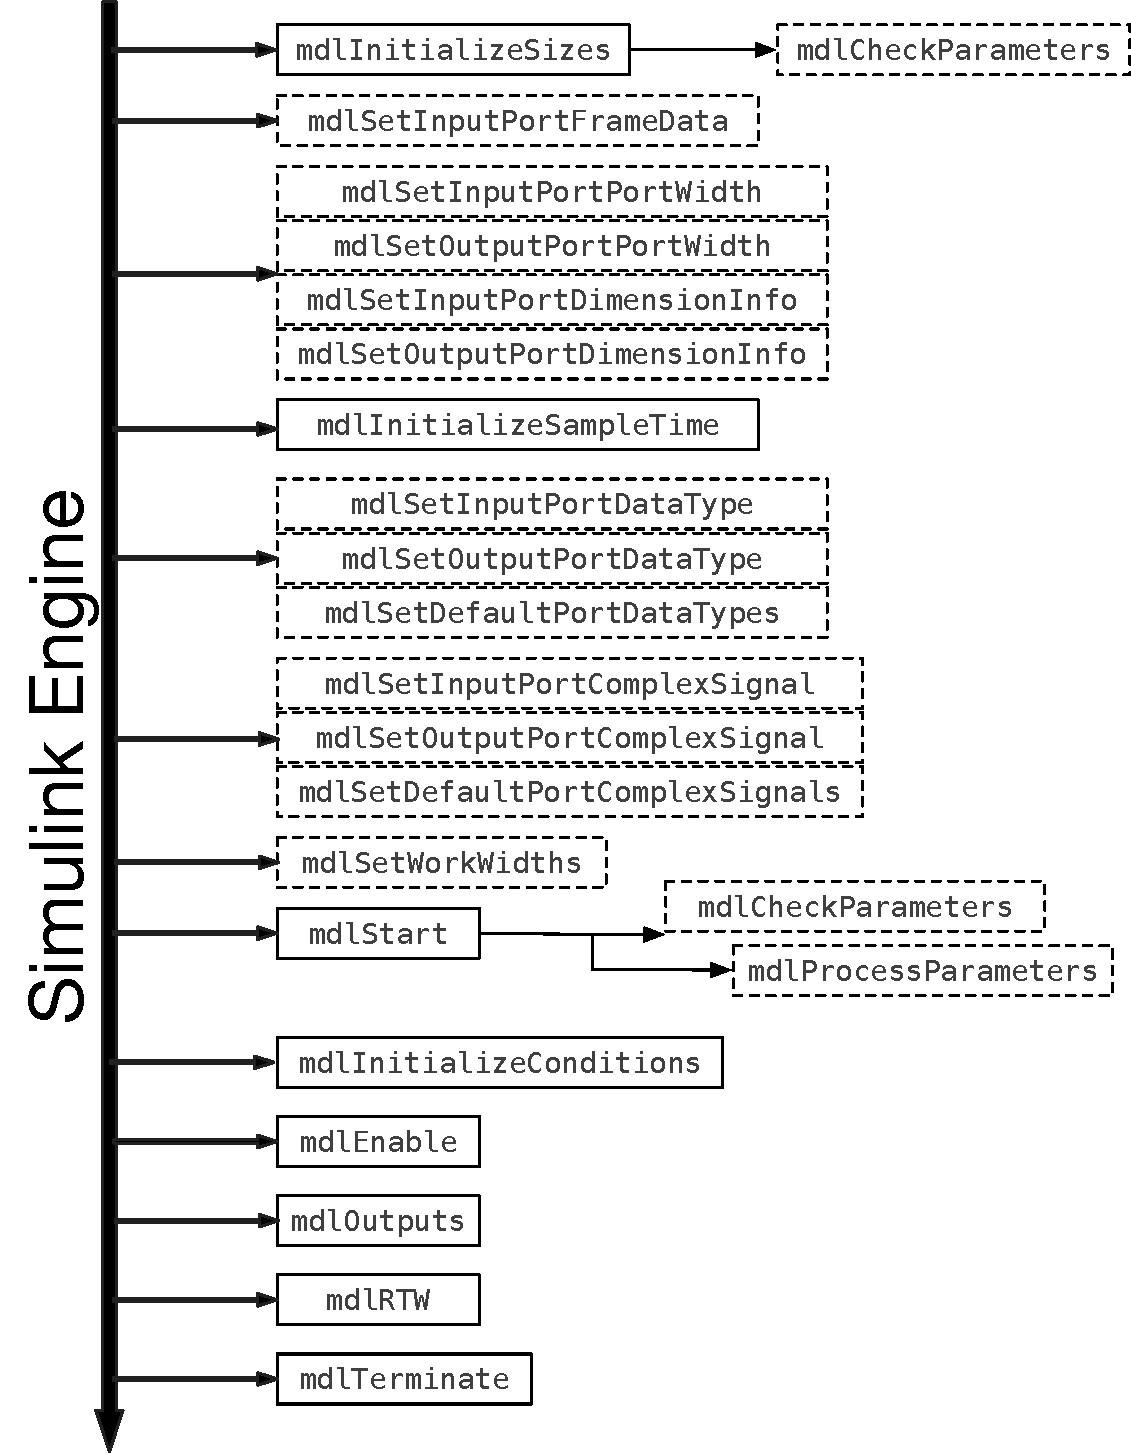
\includegraphics[width=0.8\textwidth]{RTWCallbacks}
\caption{Simulink Engine Callbacks Order in Case of Code Generation}
\label{fig:RTWCallbacks}
\end{figure}
The function \verb|mdlInitializeSizes| is important because it sets the sizes of the various signals and vectors and so can inherit the port configuration information such as the size and the data type. Then through the function \verb|mdlRTW| these parameters are written into the .rtw file to be used by the TLC file.
\par Each block has a target file that determines what code should be generated for that block \cite{BlockTLC}. Within each block target file, \emph{block functions} specify the code to be output during the start function, output function, update function, and so on. After the Code generation block initialization (i.e. \verb|BlockInstanceSetup| and \verb|BlockTypeSetup|) different TLC function generate executable code, let focus on \verb|Start| and \verb|Outputs| which are used for implementing the ports. 
\begin{itemize}
\item \emph{Start}. The code inside this function executes once and only once, therefore, it is used to instantiate a global variable for the port descriptor and to initialize it (i.e. open the port).
\item \emph{Output}. The code inside this function is placed in model's Outputs function and generate the code required to access the port.
\end{itemize}

%********************************** % Section  **************************************
\section{System Target File}\label{slexSTF}
Once the model has been adapted to the software architecture described in the configuration file, a Matlab script file scans the model start the code generation process. The script run the command \verb|rtwbuild| on every subsystem, so RTW creates a folder in the current working directory and places all the generated files. In order to drive the code generation process a \emph{custom System Target File} has been developed.% \ref{sec:RTWGenerationProcess} 
\par The custom System Target File generate C code as the default System Target File from Embedded Coder would do (see section \ref{sec:CodeArchitecture}). This is achieved by exploiting the built-in TLC script \verb|codegenentry.tlc|. The generation process is incremental, so every time a new block is encountered, some code is added to the temporary data structure that later on will be combined to form the source files. At the end of the process, when all the information about the code is known, an additional XML file is generated. The file describes the interface of the generated code, including:
\begin{itemize}
\item \emph{BuildDir}. The sub-folder of the current working directory where the source files are stored.
\item \emph{SrcFiles}. The list of all the source files.
\item \emph{Header and Body}. The header and the body of the subsystem, this are the main file implementing the subsystem code.
\item \emph{Inputs and Outputs}. The name of the structure containing the Inputs/Outputs for the subsystem code and every structure element (ports) with its name and dimension.
\item \emph{Functions}. The name of the entry point functions.
\end{itemize}
An example of a subsystem called \verb|Ctrl1Err| is the following:
\lstinputlisting{Chapters/SrcCode/Ctrl1Err.xml}
This file is required because every generation process ignores all the others, particularly, the last one, which should glue all the code to form PikeOS processes and partitions, does not know anything about the code interface of the subsystems. An alternative to the XML format might be an RTW file. The drawback of this approach is that now also the Partitions generation must be done through a TLC file and Matlab, whereas, with an XML file there is a free choice about the code generation tool. Moreover, via XML file is easier to implement a heterogeneous code generation tool.

\paragraph{} Even though any other code generation tool can be used, the Partition generation is implemented used a TLC file for seamless integration with the current workflow.

%********************************** % Section  **************************************
\section{Native Application Generation}
For generating the code of each PikeOS Process (one for each Partition), another template is required. It must take the previously generated code and transform in threads than pack them in Processes. This task is performed by another TLC script.
\par The process is driven by a Matlab script that parses every XML file that has been generated by the custom System Target File enriching them with the information stored in the configuration file. The result of this operation is the previously created class structure with additional information, i.e.:
\begin{itemize}
\item Threads
\begin{itemize}
\item Code interfaces
\item Communications
\item Affinity Mask
\item Priority
\item Partition Identifier
\end{itemize}
\item Partitions
\end{itemize}
The top level class provides a public method to export all the threads inside a given partition as RTW file. This method is useful to feed the TLC script.

\subsection{PikeOS Process Generation}\label{nativeprocess}
Every PikeOS Partition is made by the Main thread and several child threads. The main thread is loaded by the PikeOS kernel, and it is responsible for initializing all the children threads. Therefore, to implement the proposed software architecture, the main thread perform the following operations:
\begin{enumerate}
\item Lower its priority to the lowest in its partition to let child threads execute their initialization code.
\item Creates all the child threads.
\item Increase its priority to the highest in its partition.
\item Enter in an infinite loop where resume all child threads and wait for the next period activation.
\end{enumerate}
The C code implementing this behavior in PikeOS is the following:
\lstinputlisting[language=C]{Chapters/SrcCode/SimpleMain.c}
Where \verb|<AffinityMask>|, \verb|<Name>| and \verb|<Prototype>| are variable that change for each thread, like in TLC script. The functions \verb|initThread| and \verb|resumeThread| are custom functions. The first one creates a PikeOS thread and sets its affinity mask, the second one resume a thread from the STOPPED state.
\par When the main lower its priority to the lowest one, the scheduler ensures that every child thread executes its initialization code than the main execute again and elevates its priority. During normal operation, the main is the highest priority thread in the partition and resumes all the threads, therefore the scheduler ensures that no one of the child thread executes before the main has resumed all threads, so the correct behavior is satisfied.

\paragraph{} The child threads have a similar structure. Every thread:
\begin{enumerate}
\item Once created, execute the initialize function of the subsystems it refers to.
\item Move to the STOPPED state, waiting for the first activation.
\item Enters into an infinite loop where. Take all the require output from the predecessors, execute the step function of the subsystem it refers to and goes again in the STOPPED state, waiting for the next activation.
\end{enumerate}
The C code implementing this behavior is the following:
\lstinputlisting[language=C]{Chapters/SrcCode/SimpleThread.c}
As discussed before, all the threads inside a process share the same virtual memory space, so an output variable for a subsystems is a global variable that can be freely retrieved by one of it successor. This communication, referred as \emph{inter-partition communication}, might require synchronization while accessing shared resources.

\subsection{Intra-Process Communication}
Assuming a non-preemptive, FIFO priority-based scheduler and a correct priority assignment, there is no need to use any synchronization mechanism when two threads on the same core try to access a shared variable. This because the scheduler ensures that the thread with the lower priority (the reader) does not execute before the completion of the higher priority thread (the writer). When the access occurs between threads scheduled on different cores there is no guarantee about the read-write operation. There might be cases in which a reader tries to get the input variable before its predecessor wrote the last value. In this case, a synchronization mechanism must be placed to avoid it.

\subsubsection{Spinlocks}
Several synchronization mechanisms solve the inter-core communication issue, the most commonly used locks are \emph{mutexes} and \emph{semaphores}.% that keep track of the number of times it has been locked and so manage thread access when it is unlocked. 
 Both mechanisms eventually block the caller thread by moving it to the WAITING state, meaning that the next schedulable thread in the queue becomes the CURRENT thread and execute. Suppose that thread $\tau_1$ perform a lock on a mutex and moves to the WAITING state, then a thread $\tau_2$ from the READY queue is scheduled. Might happen that there is a precedence relation $\tau_1\to\tau_2$ that force $\tau_2$ to block, waiting for $\tau_1$ to complete. This can happen again with the next scheduled thread and so on. Therefore, this might lead to a sequence of threads first check if all the predecessors completed their execution and eventually blocks.
\par A mechanism that avoids this drawback is the \emph{spinlock} (already described in section \ref{sec:spinlocks}). With this mechanism the thread performs a busy-wait (basically loops) on the lock until it is unlocked, so does not move to the WAITING state. Therefore, whenever the spinlock is released, the thread is sure about the availability of all the predecessor data. This mechanism, which is very cost-effective when the thread is expected to wait for a small amount of time, does not introduce the preemption issue.
\par Therefore, the TLC script adds a call to \verb|p4_spin_lock| on every read and a \verb|p4_spin_unlock| on every write on shared variables that needs to be accessed by threads scheduled on different cores.

%********************************** % Section  **************************************
\section{Operating System Configuration Generation}
As discussed in the section \ref{sec:IntegrationProject}, the Integration Project provide a way to configure the generation of the PikeOS boot image, including all the Partitions. The Integration Project uses the file \verb|project.xml| to store all the configuration information. The generation of the whole file is complex, so, for the seek of simplicity only some XML snippets are generated. This does not lead to a loss of functionality because it is possible to develop a tool that, once an Integration Project has been generated by CODEO or the command line, can scan the \verb|project.xml| File and add programmatically the snippets. 
\par The snippets that are required are the following:
\begin{itemize}
\item Partition and Ports
\item Channels
\item Schedule Scheme
\end{itemize}
With a procedure analogue to the generation of the partitions, the workspace structure containing all the information is exported in the RTW File format and used by a TLC to generate these snippets.

\subsection{Partitions and Ports}
First and foremost Resource Partitions and and their Processes musts be defined. This is made by adding some \verb|ComponentInstance| elements as child of the \verb|ConfigurationDomainTable| tag. An example of the definition of a Resource Partition is the following:
\lstinputlisting{Chapters/SrcCode/Snippets/GroupSnippet.xml}
In this snippet all relevant information are defined, i.e. \begin{enumerate*}
\item the partition and its name (e.g. PartitionA),
\item the process belonging to this partition (e.g. ProcessA),
\item the ports and their identifier (e.g.\verb|sport_0_src|).
\end{enumerate*} In this example both the Process and the Partition are grouped in a group called \verb|Partition A| (which has no impact on the boot image creation) but it is displayed in the CODEO Project Configuration.

\paragraph{} Later on in the \verb|project.xml| File, the complete enumeration of the Resource Partitions is listed as child elements of \verb|PartitionTable|, a configuration example is:
\lstinputlisting{Chapters/SrcCode/Snippets/PartitionsSnippet.xml}
Here are defined two Resource Partitions, \verb|PartitionA| and \verb|PartitionB|.

\subsection{Channels}
Once Resource Partition and their Ports are declared, Channels must connect them allowing two Partition to communicate. For example a communication between partition $\pi_2$ and partition $\pi_3$ through ports \verb|sport_0_dst| (end point of the communication) and \verb|sport_0_src| (starting point of the communication) is the following:
\lstinputlisting{Chapters/SrcCode/Snippets/ChannelsSnippet.xml}
The \verb|Channel| tag, with its children, is a child of the tag \verb|PartitionChannelTable| in the \verb|ConnetctionTable|.

\subsection{Schedule Scheme}
The schedule scheme is used to implement the Partition Schedule. As discussed in section \ref{sec:P4Scheduler}, a Schedule Scheme is by Time Windows, each of them has an identifier, a starting time and a duration. The default scheme loaded by the kernel is called \verb|SCHED_BOOT|. An example of the schedule snippet is the following.
\lstinputlisting{Chapters/SrcCode/Snippets/ScheduleSnippet.xml}
In this schedule the remaining time after the schedule of \TP{1} and \TP{2} and before the start of a new Major Time Frame (Hyper-period) is allocated to the \TP{0}. The flag \verb|VM_SCF_PERIOD| mark that time window as the start of a new period. This flag is used by PikeOS kernel to notify the Main threads to wake up.